\documentclass[nobib]{tufte-handout}

\title{Föreläsning 11: Probabilistiska metoden $\cdot$ 1MA020}

\author[Vilhelm Agdur]{Vilhelm Agdur\thanks{\href{mailto:vilhelm.agdur@math.uu.se}{\nolinkurl{vilhelm.agdur@math.uu.se}}}}

%\date{20 februari 2023}


%\geometry{showframe} % display margins for debugging page layout

\usepackage{graphicx} % allow embedded images
  \setkeys{Gin}{width=\linewidth,totalheight=\textheight,keepaspectratio}
  \graphicspath{{graphics/}} % set of paths to search for images
\usepackage{amsmath}  % extended mathematics
\usepackage{booktabs} % book-quality tables
\usepackage{units}    % non-stacked fractions and better unit spacing
\usepackage{multicol} % multiple column layout facilities
\usepackage{lipsum}   % filler text
\usepackage{fancyvrb} % extended verbatim environments
  \fvset{fontsize=\normalsize}% default font size for fancy-verbatim environments

\usepackage{color,soul} % Highlights for text

% Standardize command font styles and environments
\newcommand{\doccmd}[1]{\texttt{\textbackslash#1}}% command name -- adds backslash automatically
\newcommand{\docopt}[1]{\ensuremath{\langle}\textrm{\textit{#1}}\ensuremath{\rangle}}% optional command argument
\newcommand{\docarg}[1]{\textrm{\textit{#1}}}% (required) command argument
\newcommand{\docenv}[1]{\textsf{#1}}% environment name
\newcommand{\docpkg}[1]{\texttt{#1}}% package name
\newcommand{\doccls}[1]{\texttt{#1}}% document class name
\newcommand{\docclsopt}[1]{\texttt{#1}}% document class option name
\newenvironment{docspec}{\begin{quote}\noindent}{\end{quote}}% command specification environment

\include{mathcommands.extratex}

\begin{document}

\definecolor{darkgreen}{rgb}{0.0627, 0.4588, 0.1451}

\maketitle% this prints the handout title, author, and date

\begin{abstract}
\noindent
I denna föreläsning ger vi fler tillämpningar av probabilistiska metoden på olika problem, praktiska och från andra delar av matematiken. Många men inte alla kommer handla om grafer.
\end{abstract}

\section{\texttt{min-bisection}-problemet}

Antag att vi har en grupp personer på en konferens, och vi vill dela upp dem i två lika stora grupper i olika rum. Vi vill att så många som möjligt som känner varandra skall få vara i samma rum -- ekvivalent vill vi alltså minimera mängden vänskapsband mellan rummen.\sidenote[][]{
  Ett annat sätt att motivera det här problemet är att vi har en graf som är för stor för att lagra i minnet på en enda dator, så vi vill använda två datorer och låta var och en av dem lagra hälften. Så länge vad vi vill räkna ut bara handlar om noder på en av de två datorerna kan vi räkna lokalt -- men om vi vill räkna ut något som involverar kanter mellan de två maskinerna måste de kommunicera med varandra, vilket är långsamt.
  
  För att kunna göra snabba beräkningar vill vi alltså hitta ett sätt att dela upp vår graf så att det inte går så många kanter mellan de två delarna. Det här är ett problem som behöver lösas i praktiken, även om man ofta då har fler än två datorer och behöver hitta en minimal $k$-partition av grafen istället.}

\begin{definition}
  Givet en graf $G = (V, E)$ på $2n$ noder är \texttt{min-bisection} problemet att hitta en minimal bisektion av $G$, alltså att hitta en delmängd $A \in \binom{V}{n}$ som minimerar antalet kanter mellan $A$ och $A^c$. Formellt skriver vi
  $$\min_{A \in \binom{V}{n}} \abs{E(A, A^c)}$$
  där $E(A, A^c)$ alltså är mängden av kanter mellan $A$ och dess komplement $A^c$.
\end{definition}

Hur väl kan vi lösa det här problemet? Ibland är det väldigt svårt -- om vi har fyra personer där alla känner alla, alltså grafen är den fullständiga grafen $K_4$, kommer vi alltid att ha $4$ av $6$ kanter mellan de två delarna.

\begin{figure}
  \centering
  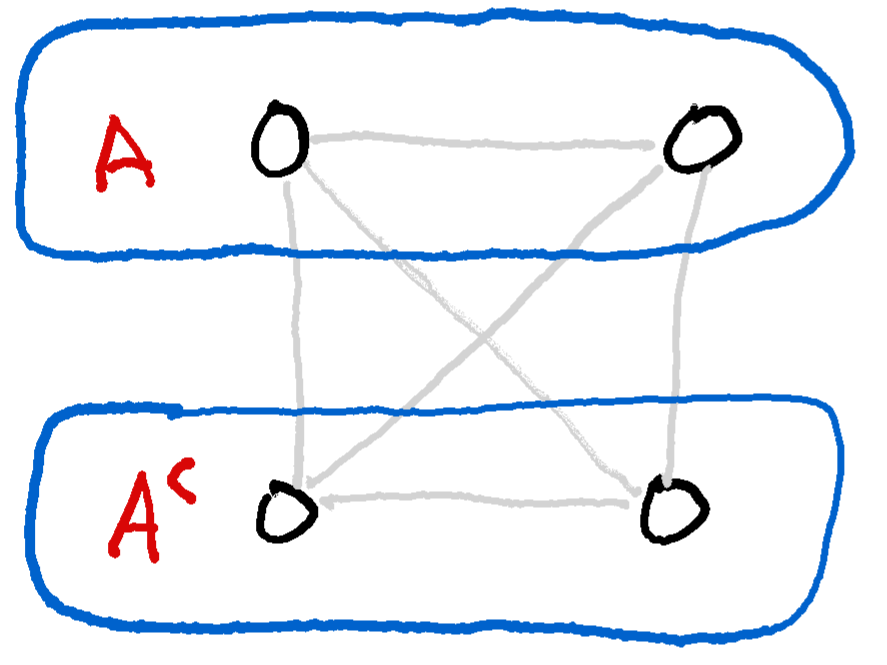
\includegraphics[width=0.5\textwidth]{graphics/K4_min_bisection.png}
  \caption{$K_4$ uppdelad i en bisektion. På grund av symmetrin i grafen är detta så klart enda sättet att dela upp den.}
\end{figure}

Det visar sig att nyckelegenskapen för att kunna göra det här väl är att grafen inte får ha för många kanter relativt antalet noder -- vilket väl inte är allt för överraskande, om man tänker efter.

För att kunna ge en precis variant av det påståendet behöver vi en definition och en sats från grafteorin.

\begin{definition}
  En Hamiltoncykel i en graf är en cykel som innehåller alla noder exakt en gång. Givet $G = ([n],E)$ kan vi alltså se det som en permutation $\sigma \in S_n$ sådan att $\{\sigma(i),\sigma(i+1)\}$ är en kant för alla $i$, och $\{\sigma(1), \sigma(n)\} \in E$.
\end{definition}

\begin{theorem}[Diracs sats]\sidenote[][]{Inte fysikern, en annan Dirac.}
  Om varje nod i $G = ([n], E)$ har grad\sidenote[][]{Antal grannar.} minst $\frac{n}{2}$ så finns det en Hamiltoncykel i $G$.

  \begin{proof}
    Hade gärna inkluderat ett, men vi har inte riktigt tid med det -- och hittade inget probabilistiskt bevis för detta, så det passar inte helt.
  \end{proof}
\end{theorem}

Vi kan använda denna sats för att bevisa följande resultat:

\begin{proposition}
  Låt $G = ([n], E)$ vara en graf på ett jämnt antal noder, och antag att varje nod har grad högst $\frac{n}{2}$. Då existerar det en delmängd $A \in \binom{[n]}{n/2}$ sådan att
  $$E(A, A^c) \leq \frac{\abs{E}}{2}.$$ 

  \begin{proof}
    Låt $G'$ vara komplementgrafen till $G$ -- alltså grafen där det finns en kant mellan varje par av noder som \emph{inte} har en kant mellan sig i $G$, och som inte har en kant mellan par av noder som har en kant i $G$.

    Vi ser enkelt att graden av $i$ i $G'$ är precis $n$ minus graden av $i$ i $G$, så eftersom $d_i \leq n/2$ i $G$ måste $d_i' \geq n/2$ i $G'$. Alltså kan vi tillämpa Diracs sats och hitta en Hamiltoncykel $\sigma$ i komplementgrafen $G'$.

    Vi kan nu använda denna Hamiltoncykel för att para ihop noder i $G$ -- vi matchar $\sigma(1)$ med $\sigma(2)$, $\sigma(3)$ med $\sigma(4)$, och så vidare. Eftersom detta var en Hamiltoncykel i komplementgrafen är vi alltså garanterade att vi aldrig parar ihop två noder som har en kant mellan sig.

    Vi kan nu skapa oss en slumpmässig delmängd $A \in \binom{[n]}{n/2}$ genom att, för varje par, slumpmässigt välja en av de två noderna att ha med i $A$, och låta den andra vara utanför $A$. Denna delmängd kommer ha rätt storlek eftersom vi väljer en nod ur varje par, så vi måste få precis hälften av noderna.

    Låt oss nu räkna ut väntevärdet av $E(A, A^c)$. Vi får att
    \begin{align*}
      \E{E(A, A^c)} &= \E{\sum_{e \in E} \ind{e \in E(A, A^c)}}\\
      &= \sum_{e \in E} \E{\ind{e \in E(A, A^c)}}\\
      &= \sum_{e \in E} \Prob{e \in E(A, A^c)}.
    \end{align*}

    Vad är sannolikheten att en viss fix kant $e = \{u, v\}$ går mellan $A$ och $A^c$? Jo, det händer precis när vi valt att $u \in A$ och $v \in A^c$, eller vice versa. Så vi kan räkna att\sidenote[][]{Vi utnyttjar att de är disjunkta händelser för att gå från $\Prob{(u \in A, v \in A^c) \cup (u \in A^c, v \in A)}$ till summan av de två sannolikheterna.}
    $$\Prob{\{u,v\} \in E(A, A^c)} = \Prob{u \in A, v \in A^c} + \Prob{u \in A^c, v \in A}.$$
    
    Nyckeln nu, och anledningen att vi krånglade med Hamiltoncykeln och hopparningen, är att händelserna $u\in A$ och $v\in A^c$ måste vara oberoende. Om $u$ är i $A$ eller inte beror på en myntsingling vi gjorde för $u$ och noden den parades ihop med -- så om vi kallar dess partner för $w$ så är $u \in A$ och $w \in A$ inte oberoende, men för alla $v \neq w$ är $u \in A$ oberoende från $v \in A$.

    Så hur vet vi att vårt par $u, v$ i vår räkning inte råkar vara hopparade, så att det inte är oberoende ifall de ligger i $A$ eller ej? Jo, vi vet ju att det går en kant mellan $u$ och $v$ -- det är därför vi är intresserade av dem -- men det går ingen kant mellan något par av hopparade noder.

    Alltså kan vi fortsätta vår räkning och få
    \begin{align*}
      \Prob{\{u,v\} \in E(A, A^c)} &= \Prob{u \in A, v \in A^c} + \Prob{u \in A^c, v \in A}\\
      &= \Prob{u \in A}\Prob{v \in A^c} + \Prob{u \in A^c}\Prob{v \in A}\\
      &= \frac{1}{2}\cdot\frac{1}{2} + \frac{1}{2}\cdot\frac{1}{2} = \frac{1}{2}
    \end{align*}
    och alltså har vi att
    \begin{align*}
      \E{E(A,A^c)} &= \sum_{e \in E} \Prob{e \in E(A, A^c)}\\
      &= \sum_{e \in E} \frac{1}{2} = \frac{\abs{E}}{2}.
    \end{align*}

    Enligt vårt sedvanliga argument att väntevärdet omöjligen kan vara mindre än varje specifikt utfall måste det alltså finnas ett specifikt $A$ sådant att $E(A, A^c) \leq \E{E(A,A^c)} = \frac{\abs{E}}{2}$ och vi har bevisat satsen.
  \end{proof}
\end{proposition}

\section{ACNSL-olikheten och VLSI}

\section{Oberoende mängder i triangelfria grafer}

\section{Längsta ökande delföljden i en permutation}

\section{Övningar}


%\bibliography{references}
%\bibliographystyle{plainnat}

\end{document}
